Проверяющий модуль делает следующий вызов функции:

\texttt{find\_best(8)}

Используются $n = 8$ коробок со следующими типами призов $[3,2,3,1,3,3,2,3]$. Все
возможные вызовы функции \texttt{ask} и возвращаемые значения перечислены ниже

\begin{itemize}
\item `ask(0)' возвращает $[0, 3]$
\item `ask(1)' возвращает $[0, 1]$
\item `ask(2)' возвращает $[1, 2]$
\item `ask(3)' возвращает $[0, 0]$
\item `ask(4)' возвращает $[2, 1]$
\item `ask(5)' возвращает $[2, 1]$
\item `ask(6)' возвращает $[1, 0]$
\item `ask(7)' возвращает $[3, 0]$
\end{itemize}

В этом примере бриллиант находится в коробке с номером $3$. Возвращаемое значение
функции \texttt{find\_best} должно быть равно $3$.

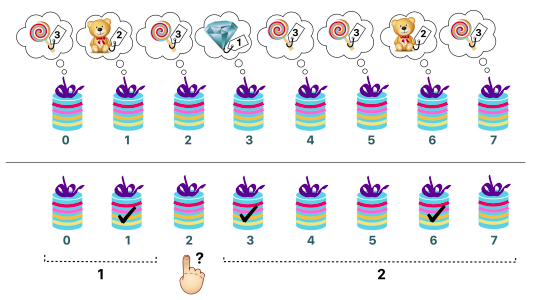
\includegraphics{prize.png} 

Рисунок выше иллюстрирует пример. Верхняя часть показывает значения типов призов в
каждой из коробок. Нижняя часть иллюстрирует вызов \texttt{ask(2)}, отмеченные коробки содержат более дорогие, чем приз из коробки с номером $2$.